\documentclass[12pt]{article}
\usepackage{geometry} % Pour passer au format A4
\geometry{hmargin=1cm, vmargin=2cm} % 

% Page et encodage
\usepackage[T1]{fontenc} % Use 8-bit encoding that has 256 glyphs
\usepackage[english,french]{babel} % Français et anglais
\usepackage[utf8]{inputenc} 

\usepackage{lmodern}
\setlength\parindent{0pt}


\usepackage{fourier}
%\usepackage[scaled=0.875]{helvet} 
\renewcommand{\ttdefault}{lmtt} 
\usepackage{amsmath,amssymb,makeidx}
\usepackage[normalem]{ulem}
\usepackage{fancybox,graphicx}
\usepackage{tabularx,booktabs}
\usepackage{pifont}
\usepackage{ulem}
\usepackage{dcolumn}
\usepackage{textcomp}
\usepackage{diagbox}
\usepackage{tabularx}
\usepackage{multirow,multicol}
\usepackage{lscape}
\newcommand{\euro}{\eurologo{}}

%Tapuscrit : François Kriegk
\usepackage{pst-eucl}
\usepackage{diagbox}% à mettre après pst-eucl
\usepackage{graphicx,pstricks,pst-plot,pst-grad,pst-node,pst-text,pstricks-add}
\usepackage{pgf,tikz,pgfplots}
\usetikzlibrary{patterns,calc,decorations.pathmorphing}
\setlength\paperheight{297mm}
\setlength\paperwidth{210mm}
\setlength{\textheight}{25cm}
\newcommand{\R}{\mathbb{R}}
\newcommand{\N}{\mathbb{N}}
\newcommand{\D}{\mathbb{D}}
\newcommand{\Z}{\mathbb{Z}}
\newcommand{\Q}{\mathbb{Q}}
\newcommand{\C}{\mathbb{C}}

\renewcommand{\theenumi}{\textbf{\arabic{enumi}}}
\renewcommand{\labelenumi}{\textbf{\theenumi.}}
\renewcommand{\theenumii}{\textbf{\alph{enumii}}}
\renewcommand{\labelenumii}{\textbf{\theenumii.}}

\newcommand{\vect}[1]{\mathchoice%
  {\overrightarrow{\displaystyle\mathstrut#1\,\,}}%
  {\overrightarrow{\textstyle\mathstrut#1\,\,}}%
  {\overrightarrow{\scriptstyle\mathstrut#1\,\,}}%
  {\overrightarrow{\scriptscriptstyle\mathstrut#1\,\,}}}
\def\Oij{$\left(\text{O},~\vect{\imath},~\vect{\jmath}\right)$}
\def\Oijk{$\left(\text{O},~\vect{\imath},~\vect{\jmath},~\vect{k}\right)$}
\def\Ouv{$\left(\text{O},~\vect{u},~\vect{v}\right)$}
\setlength{\voffset}{-1,5cm}

\usepackage{fancyhdr} 
\pagestyle{fancyplain} 

\fancyhead{} % No page header
\fancyfoot{}

\renewcommand{\headrulewidth}{0pt} % Remove header underlines
\renewcommand{\footrulewidth}{0pt} % Remove footer underlines

\newcommand{\horrule}[1]{\rule{\linewidth}{#1}} % Create horizontal rule command with 1 argument of height

\newcommand{\tempsexo}[1]{\textit{\textbf{(#1)}}}
%----------------------------------------------------------------------------------------
%   Début du document
%----------------------------------------------------------------------------------------

\begin{document}

%----------------------------------------------------------------------------------------
% RE-DEFINITION
%----------------------------------------------------------------------------------------
% MATHS
%-----------

\newtheorem{Definition}{Définition}
\newtheorem{Theorem}{Théorème}
\newtheorem{Proposition}{Propriété}

% MATHS
%-----------
\renewcommand{\labelitemi}{$\bullet$}
\renewcommand{\labelitemii}{$\circ$}
%----------------------------------------------------------------------------------------
%   Titre
%----------------------------------------------------------------------------------------

\setlength{\columnseprule}{1pt}

\section*{S2 : Semaine du 23/03 au 29/03 - Exercice complémentaire}

\begin{itemize}
  \item Brevet 2019 - La Réunion Antilles-Guyane
  \item 8 points
  \item 5 / 15 minutes pour l'exercice
  \item 5 minutes pour la lecture et la compréhension de la correction
\end{itemize}

 \horrule{2px}

\parbox{0.8\linewidth}{
    Hugo réalise un assemblage de carreaux représentant son héros préféré. \\
    Pour cela il doit coller 22 carreaux violets, 2 blancs, 162 noirs et 110 verts.\\
    Tous les carreaux sont mélangés dans une boîte.\\
    Hugo choisit un carreau au hasard.\\
    On estime que tous les carreaux ont la même chance d'être choisis.\\

    \medskip
    \begin{enumerate}
    \item Quelle est la probabilité que Hugo choisisse un carreau vert ?
    \item Quelle est la probabilité que Hugo ne choisisse pas un carreau violet ?
    \item Quelle est la probabilité que le carreau choisi soit noir ou blanc?
    \item En une journée Hugo a collé 75\,\% des carreaux. Combien de carreaux cela représente-t-il ?
    \end{enumerate}
    }
\hfill \parbox{0.18\linewidth}{
    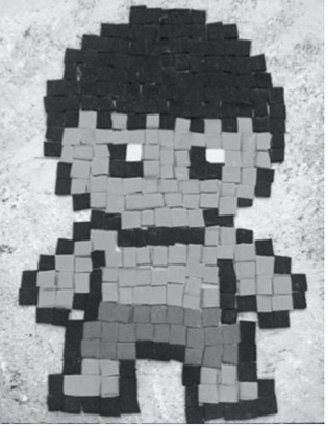
\includegraphics[width=3cm]{_continuite/sources/s3-heros.pdf}
    }

\newpage

\section*{Correction}

\begin{enumerate}
    \item Il y a 110 carreaux verts sur un total de $22 + 2 + 162 + 110 = 296$ carreaux. \\
    La probabilité de tirer un carreau vert est égale à $\dfrac{110}{296} = \dfrac{55}{148}$.
    \item La probabilité de choisir un carreau violet est $\dfrac{22}{296} = \dfrac{11}{148}$, donc la probabilité de ne pas choisir un carreau violet est $1 - \dfrac{11}{148} = \dfrac{148 - 11}{148} = \dfrac{137}{148}$.
    \item La probabilité que le carreau choisi soit noir ou blanc est $\dfrac{162 + 2}{296} = \dfrac{164}{296} = \dfrac{41}{74}$.
    \item On a $\dfrac{75}{100} \times 296 = \dfrac{22200}{100} = 222$. \\
    Hugo a collé 222 carreaux en une journée.
\end{enumerate}


\end{document}